\documentclass{anstrans}

\title{SUMMARY TITLE}
\author{Sun Myung Park}
\institute{Dept. of Nuclear, Plasma and Radiological Engineering, University of Illinois at Urbana-Champaign \\
smpark3@illinois.edu}

\usepackage{graphicx} % allows inclusion of graphics
\usepackage{booktabs} % nice rules (thick lines) for tables
\usepackage{microtype} % improves typography for PDF
\usepackage{xspace}
\usepackage{multirow} 
\usepackage{array}
\setlength{\arrayrulewidth}{.4mm}
\renewcommand{\arraystretch}{1.2}
\usepackage[labelfont=bf]{caption}
\captionsetup[table]{name=Table}
\renewcommand{\thetable}{\arabic{table}}
\usepackage{subcaption}
\usepackage{enumitem}
\usepackage{placeins}
\newcolumntype{c}{>{\hsize=.56\hsize}X}
\newcolumntype{b}{>{\hsize=.7\hsize}X}
\newcolumntype{s}{>{\hsize=.74\hsize}X}
\newcolumntype{f}{>{\hsize=.1\hsize}X}
\newcolumntype{a}{>{\hsize=.45\hsize}X}
\usepackage{titlesec}
\titleformat*{\subsection}{\normalfont}

\begin{document}

\section{INTRODUCTION}

Moltres is an open source simulation tool developed for simulating MSRs. It is an application code that is developed in Multiphysics Object Oriented Simulation Environment (MOOSE) \cite{gaston_moose:_2009}, a finite-element, multi-physics framework for solving non-linear problems. Through the MOOSE framework, Moltres solves the coupled n-group neutron diffusion, temperature and delayed neutron precursor governing equations on a coarse, adaptive meshing scheme. 

A demonstration of Moltres has been performed by Lindsay et al. \cite{lindsay_introduction_2018} with the Molten Salt Reactor Experiment (MSRE) reactor design developed by Oak Ridge National Laboratory in the 1950s and 60s. In that paper, a 2D-axisymmetric model resembling the MSRE design was simulated on Moltres for proof-of-concept, followed by a 3D geometry also resembling the MSRE design. The temperature and neutron flux results from the 3D model were found to be in good agreement with analytical solutions for the MSRE by Briggs et al. \cite{briggs_molten-salt_1964}. Moltres can also be easily coupled with other MOOSE application codes for additional physics to be introduced into MSR simulations.

\section{MOTIVATION}

The logical next step in the development of Moltres is its application on other MSR designs. The MSR design of interest for this summary and the subsequent report is the Molten Salt Fast Reactor (MSFR) \cite{serp_molten_2014}. The pool-type MSFR is a fast reactor that consists of a single large pool of fuel-containing molten salt flowing upwards through the center of the core, which later separates into 16 smaller coolant loops for heat exchange, pumping and other processes before flowing back into the center. As a fast reactor, it has no need for numerous graphite moderator channels such as those found in the channel-type epithermal reactor of the MSRE.

There are a number of technological gaps in the Moltres code that have to be filled in order to accurately simulate the physics present in the MSFR, especially for transient and accident scenarios. Some features that will be developed include improvements in the fluid dynamics, as Moltres can currently only handle laminar flow at predetermined velocity distributions.

\section{BACKGROUND OF MOLTEN SALT REACTORS}

%A major feature to be introduced is pump and buoyancy driven flow. The current implementation of Moltres requires user-determined velocity values as opposed to having the flow determined by fluid dynamics in the presence of pumps and buoyancy effects due to the expansion of heated molten salt. While this implementation is sufficient for 

Molten salt reactors (MSR) were first developed in the 1950s and 60s as part of the Aircraft Reactor Experiment (ARE) and later the Molten Salt Reactor Experiment (MSRE) at Oak Ridge National Laboratory (ORNL). A breeder version of the MSRE design was conceptualized but never operated as funding was cut in favour of liquid metal fast-breeder reactors (LMFBR) \cite{macpherson_molten_1985}.

There has been a revival of interest in MSRs at the turn of the century, especially as the MSR is one of six advanced reactor designs shortlisted by the Generation IV International Forum (GIF) \cite{doe_technology_2002}. The GIF aims to coordinate and support research efforts into these next generation nuclear power designs. The six designs boast improvements over existing reactor systems in various factors including safety, energy efficiency, sustainability and cost \cite{doe_technology_2002}. As the name suggests, MSRs uniquely feature fuel directly dissolved in molten salt coolants as opposed to solid fuel forms that are physically separate from the coolant. Thus, MSRs may behave very differently in comparison to other reactor designs, and these differences have a big impact on the safety and operation of MSRs. New simulation tools are required to account for the different types of physical phenomena present in MSRs, such as delayed neutron precursor drifts in the molten salt.

MSRs are arguably much safer than conventional nuclear reactors due to several passive safety mechanisms that make severe accidents extremely unlikely to occur. When core temperatures rise due to unprotected reactivity insertions, the strong negative temperature reactivity coefficients of the fuel salt limit further increases in reactivity and temperature \cite{elsheikh_safety_2013}. The coolant salts are chemically inert and do not react explosively with air or water. Fission products can be continuously removed through online chemical reprocessing and helium sparging. This reduces the radiological impact of a severe accident involving a hull breach and the release of molten salt to the environment \cite{elsheikh_safety_2013}.

Certain MSR designs also operate with epithermal or fast neutron spectra which can be utilised to burn off transuranic elements which are inevitably produced when using $^{235}$U fuel. Some designs such as the Molten Salt Fast Reactor (MSFR) are designed to breed fissile $^{233}$U from $^{232}$Th \cite{serp_molten_2014}, thereby gaining the advantages of running a thorium fuel cycle. The thorium fuel cycle is stated to be more sustainable than the uranium fuel cycle due to the greater relative abundance of natural thorium resources \cite{iaea_thorium_2005}. MSRs also typically operate at low pressures compared to light water reactors (LWR) as the operating temperatures are far below the boiling temperatures of the molten salt mixture. This eliminates the need for thick pressure vessels borne from safety constraints \cite{elsheikh_safety_2013}.

\section{MOLTEN SALT FAST REACTOR}

The MSFR is a reference design for a fast-spectrum molten salt reactor first developed under the Evaluation and Viability of Liquid Fuel Fast Reactor System (EVOL) project and continued by the Safety Assessment of the Molten Salt Fast Reactor (SAMOFAR) project \cite{serp_molten_2014}. Figure \ref{fig:msfr} shows a schematic view of the MSFR. The main specifications of the MSFR are given in Table \ref{table:msfr}.

\begin{figure}[t] 
	\centering
	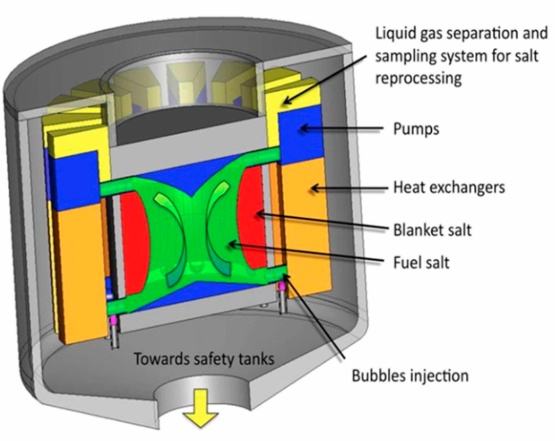
\includegraphics[width=0.48\textwidth]{./figures/MSFR}
	\caption{MSFR reactor design concept \cite{serp_molten_2014}.}
	\label{fig:msfr}
\end{figure} 

\begin{table}
\begin{tabular}{ l l }
Parameter & Value \\
\hline
Thermal/Electric power [MW$_{\text{th}}$/MW$_{\text{e}}$] & 3000 / 1300  \\
Salt volume [m$^3$] & 18 \\
Salt fraction in core & 0.5 \\
Number of circulation loops & 16 \\
Nominal flow rate [kg s$^{-1}$] & 18500  \\
Nominal circulation time [s] & 4.0 \\
Inlet/outlet temperature [K] & 973 / 1073 \\
Blanket volume [m$^3$] & 7.3
\end{tabular}
\caption{Specifications of the MSFR design \cite{serp_molten_2014}.}
\label{table:msfr}
\end{table}

The major component of the fuel and blanket molten salts used for the MSFR is lithium fluoride (LiF). Fissile and fertile isotopes are introduced into the mixture by mole fractions of 77.5\%LiF-22.5\%AcF$_4$, where AcF$_4$ represents actinide fluorides such as uranium and thorium fluorides. The MSFR supports various fuel compositions. It can run on same $^{235}$U-$^{238}$U fuel used in most conventional LWRs. It can also be run on a mixture of fresh uranium fuel with transuranic isotopes in used fuel that has been reprocessed \cite{fiorina_investigation_2013}. However, the main configuration of the MSFR is a breeder reactor running on $^{233}$U-$^{232}$Th \cite{merle-lucotte_launching_2011}. Breeding ratios of up to 1.1 have been reported by previous studies on the MSFR \cite{fiorina_molten_2013}. 

The MSFR consists of a central core region of volume 9 m$^3$. The primary fuel salt flows upwards through this region and then later separates into 16 smaller external loops, where it passes through the heat exchanger and is pumped back into the core. The primary heat exchangers transfer heat from the fuel salt to an intermediate salt coolant loop. There are other instrumentation along the external loops for online reprocessing and gas sparging. The core is radially surrounded by a tank of blanket molten salt, with reflectors at the top and bottom of the core. The blanket salt contains fertile isotopes such as $^{232}$Th for fuel breeding. There is a layer of neutron absorbing material behind the blanket tanks to protect the heat exchangers, pumps and other instrumentation from neutron irradiation damage.

A number of steady state and transient multiphysics simulations have been performed and studied for the MSFR. A paper by Fiorina et al. \cite{fiorina_modelling_2014} compares results between coupled models developed on the multiphysics code COMSOL and an in-house code developed at Delft University of Technology. The models used 2D axisymmetric models of the MSFR and solved multi-group neutron diffusion equations for the neutronics, and they showed good agreement for some of the transient cases studied. A more comprehensive 3D model has been developed and studied by Aufiero et al. \cite{aufiero_development_2014} using the computional fluid dynamics (CFD) toolbox OpenFOAM. Although this model relied on the one-group neutron diffusion equation, it enabled the study of the full 3D core geometry and 3D transient scenarios such as the failure of one of the 16 pumps in the MSFR.

More recently, a coupled tool, comprising of the thermal-hydraulics code TRACE and a multi-group 3D spatial neutronics solver PARCS, was used to run steady state and transient simulations of the MSFR \cite{pettersen_coupled_2016}. This approach allowed for a 3D model simulation of the MSFR on a coarse mesh, thus improving on the 2D axisymmetric COMSOL/TUDelft models with the benefit of much lower computation times in comparison to the CFD-OpenFOAM models. 

\section{SIMULATION CODE}

Moltres is an application code developed in the MOOSE framework \cite{gaston_moose:_2009}. The MOOSE framework solves non-linear equations through the discretization of partial differential equations (PDE) on an adaptive coarse meshing scheme provided by LibMesh \cite{kirk_libmesh:_2006} and PetSc \cite{satish_balay_petsc_2015}. Individual terms of PDEs that define the physics involved in a system are represented in MOOSE (and its applications) by kernels. For example, the various terms in the neutron diffusion equation such as the diffusion term, time evolution term, etc. all have a corresponding physics kernel defined in Moltres. Boundary conditions are also handled in a similar fashion. Moltres can solve for an arbitrary number of neutronics groups as long as the relevant group constants are provided in a Moltres-compatible format.

\begin{table*}[t]
\centering
\begin{tabular}{ l | l | l | l | l | l | l }
Group number & 1 & 2 & 3 & 4 & 5 & 6\\
\hline
Neutron energy upper bound [MeV] & 7.485$\times 10^{-4}$ & 5.5308$\times 10^{-3}$ &  2.47875$\times 10^{-2}$ & 0.4979 & 2.2313 & System maximum
\end{tabular}
\caption{Neutron energy upper bounds used in Serpent and SCALE.}
\label{table:bound}
\end{table*}

As mentioned in the previous Moltres study \cite{lindsay_introduction_2018}, the neutronics in Moltres is described by the time-independent multi-group neutron diffusion equation as shown in Equation \ref{eq1}.
\begin{align}
\frac{1}{v_g} &\frac{\partial \phi_g}{\partial t} - \nabla \cdot D_g \nabla \phi_g + \Sigma^r_g \phi_g \nonumber \\ 
&= \sum^G_{g \neq g'} \Sigma^s_{g' \rightarrow g} \phi_{g'} + \chi^p_g \sum^G_{g'=1} (1-\beta) \nu \Sigma^f_{g'} \phi_{g'} + \chi^d_g \sum^I_i \lambda_i C_i \label{eq1}
\end{align}
The delayed neutron precursors are governed by the following equation:
\begin{align}
\frac{\partial C_i}{\partial t} = \sum^G_{g'=1} \beta_i \nu \Sigma^f_{g'} \phi_{g'} - \lambda_i C_i - \frac{\partial}{\partial z} u C_i \label{eq2}
\end{align}
Lastly, the governing equation for temperature in the molten salt is given by:
\begin{align}
\rho_f c_{p,f} \frac{\partial T_f}{\partial t} + \nabla \cdot \big( \rho_f c_{p,f} \overrightarrow{u} \cdot T_f - k_f \nabla T_f \big) = Q_f \label{eq3}
\end{align}
where the source term $Q_f$ is given as:
\begin{align}
Q_f = \sum^G_{g=1} \epsilon_{f,g} \Sigma_{f,g} \phi_g \label{eq4}
\end{align}
The governing equation for temperature in the structural components is similar to that for the molten salt, with exclusion of the advection term.
\begin{align}
\rho_s c_{p,s} \frac{\partial T_s}{\partial t} + \nabla \cdot \big(- k_s \nabla T_s \big) = Q_s \label{eq5}
\end{align}
Further research will be conducted to determine the mathematical form of $Q_s$, which is the source term in the structural components due to gamma and neutron irradiation upon these components.

The group constants are to be generated on Serpent \cite{leppanen_serpent_2015} and SCALE \cite{dehart_reactor_2011}. The group constant data generated by these two codes may not necessarily agree due to differences in their implementation; Serpent is a Monte Carlo code while SCALE has both deterministic and Monte Carlo transport capabilities separately. Thus, an analysis of the two codes will be conducted to determine which set of data is more appropriate for the MSFR.

\section{METHODOLOGY}

An established benchmark reactor core geometry is used in this study. It is a 2D axisymmetric model resembling the MSFR as shown in Figure \ref{fig:benchmark}. This facilitates comparisons with previous MSFR studies by various authors \cite{fiorina_modelling_2014} \cite{pettersen_coupled_2016} on the same geometry for code validation of Moltres. Furthermore, the MSFR is still under active development and the actual geometry is expected to undergo numerous revisions with input from newer research. More complex geometries may be considered for future research. The 2D model is extended into a 3D geometry by rotating it along the central axis to form concentric cylinders, as was done by Pettersen \cite{pettersen_coupled_2016}.

Six-group neutronics data will be obtained from both Serpent and SCALE. The input consists of the 3D benchmark geometry, material properties of the various components in the MSFR, the neutron energy bounds, and the temperatures at which the group constants are to be generated. Serpent is a continuous-energy Monte Carlo neutronics solver which can run on 3D geometries. As for SCALE, the NEWT module is a 2D deterministic neutronics code while the KENO module is a 3D Monte Carlo code, like Serpent (gotta double check with Andrei/SCALE manual). An analysis will be conducted to determine which of these codes produce the group constants data that is most appropriate for the MSFR benchmark model. 

The temperatures at which the neutronics solvers are run range from 900 K to 1200 K at 50 K intervals. This range covers the normal operating temperature range of the MSFR. Preliminary Serpent results are available and discussed in the next section.

Moltres automatically interpolates the temperature-specific group constants data that it is provided, such as the various neutron cross sections, in order to possess data for all temperature values in the range of 900 K - 1200 K. 

\begin{figure}[t] 
	\centering
	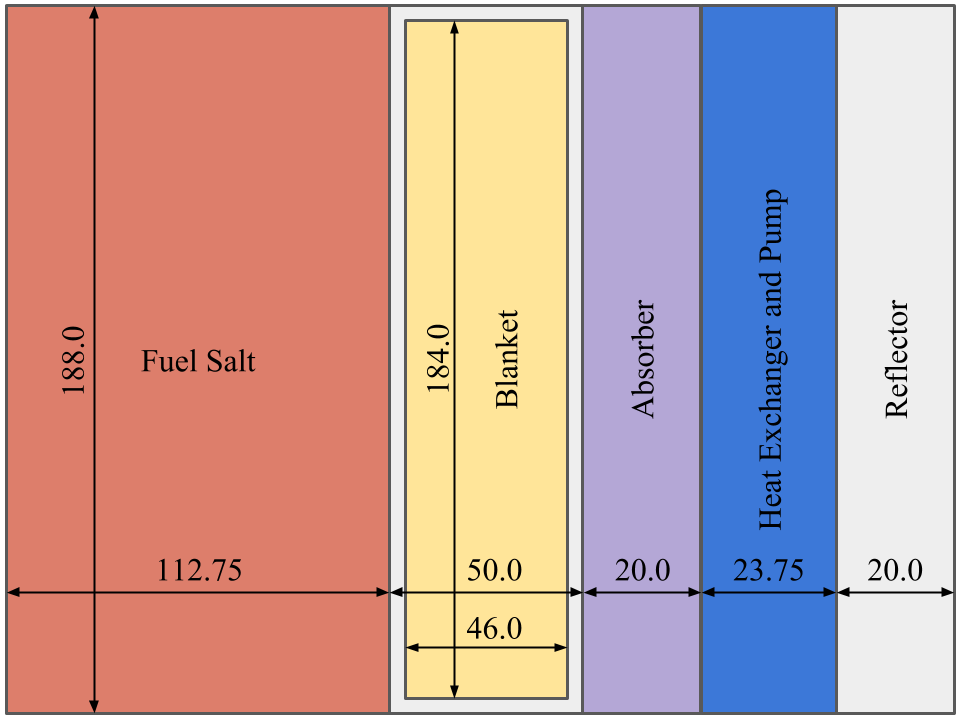
\includegraphics[width=0.48\textwidth]{./figures/benchmark}
	\captionsetup{justification=centering}
	\caption{Cross-section of the 2D axisymmetric benchmark model of the MSFR \cite{pettersen_coupled_2016}. The figure is not to scale.}
	\label{fig:benchmark}
\end{figure} 

\section{PRELIMINARY SERPENT NEUTRONICS RESULTS}

\noindent [Insert Serpent results and compare keff with Pettersen's results]

\bibliographystyle{ans}
\bibliography{bibliography}

\end{document}
